
\documentclass[sigconf]{acmart}

\usepackage{csquotes}
\usepackage{balance}
\usepackage[super]{nth}
\usepackage[binary-units=true]{siunitx}

\makeatletter
\def\etal{\textit{et~al}.~}
\def\eg{e.g., } 
\def\ie{i.e., } 
\def\cf{cf. } 
\def\wrt{w.r.t. } 
\def\etc{etc. } 
\def\vs{vs. }
\makeatother

\setcopyright{acmcopyright}

\copyrightyear{2019} 
\acmYear{2019} 
\acmConference[VINCI'2019]{The 12th International Symposium on Visual Information Communication and Interaction}{September 20--22, 2019}{Shanghai, China}
\acmBooktitle{The 12th International Symposium on Visual Information Communication and Interaction (VINCI'2019), September 20--22, 2019, Shanghai, China}
\acmPrice{15.00}
\acmDOI{10.1145/3356422.3356444}
\acmISBN{978-1-4503-7626-6/19/09}

\usepackage{eso-pic}
\AddToShipoutPictureFG{\AtPageLowerLeft{\put(\LenToUnit{0.5\paperwidth},\LenToUnit{6mm}){\makebox[0pt][c]{\fontsize{6.5}{8}\selectfont\color{gray}Author's revised version (2026-11-13). Version of record: \url{https://doi.org/10.1145/3356422.3356444}}}}}
\begin{document}

\title{Advanced Visual Metaphors and Techniques for Software Maps}

\author{Daniel Limberger}
\orcid{0000-0002-9111-4809}
\affiliation{%
  \institution{Hasso Plattner Institute, Faculty of Digital Engineering, \\University of Potsdam, Germany}
}
\email{daniel.limberger@hpi.de}

\author{Willy Scheibel}
\orcid{0000-0002-7885-9857}
\affiliation{%
  \institution{Hasso Plattner Institute, Faculty of Digital Engineering, \\University of Potsdam, Germany}
}
\email{willy.scheibel@hpi.de}

\author{J{\"u}rgen D{\"o}llner}
\orcid{0000-0002-8981-8583}
\affiliation{%
  \institution{Hasso Plattner Institute, Faculty of Digital Engineering, \\University of Potsdam, Germany}
}
\email{juergen.doellner@hpi.de}

\author{Matthias Trapp}
\orcid{0000-0003-3861-5759}
\affiliation{%
  \institution{Hasso Plattner Institute, Faculty of Digital Engineering, \\University of Potsdam, Germany}
}
\email{matthias.trapp@hpi.de}

\renewcommand{\shortauthors}{Limberger, Scheibel, D{\"o}llner, and Trapp}

\begin{abstract}
  Software maps provide a general-purpose interactive user interface and information display for software analytics tools.
  This paper systematically introduces and classifies software maps as a treemap-based technique for software cartography.
  It provides an overview of advanced visual metaphors and techniques, each suitable for interactive visual analytics tasks, that can be used to enhance the expressiveness of software maps.
  Thereto, the metaphors and techniques are briefly described, located within a visualization pipeline model, and considered within the software map design space.
  Consequent applications and use cases w.r.t. different types of software system data and software engineering data are discussed, arguing for a versatile use of software maps in visual software analytics.
\end{abstract}

\begin{CCSXML}
	<ccs2012>
	<concept>
	<concept_id>10003120.10003145.10003146.10010889</concept_id>
	<concept_desc>Human-centered computing~Treemaps</concept_desc>
	<concept_significance>500</concept_significance>
	</concept>
	<concept>
	<concept_id>10003120.10003145.10003147.10010923</concept_id>
	<concept_desc>Human-centered computing~Information visualization</concept_desc>
	<concept_significance>300</concept_significance>
	</concept>
	<concept>
	<concept_id>10003120.10003145.10011770</concept_id>
	<concept_desc>Human-centered computing~Visualization design and evaluation methods</concept_desc>
	<concept_significance>300</concept_significance>
	</concept>
	</ccs2012>
\end{CCSXML}

\ccsdesc[500]{Human-centered computing~Treemaps}
\ccsdesc[300]{Human-centered computing~Information visualization}
\ccsdesc[300]{Human-centered computing~Visualization design and evaluation methods}

\keywords{treemap, design space, information visualization}

\begin{teaserfigure}
  \centering
  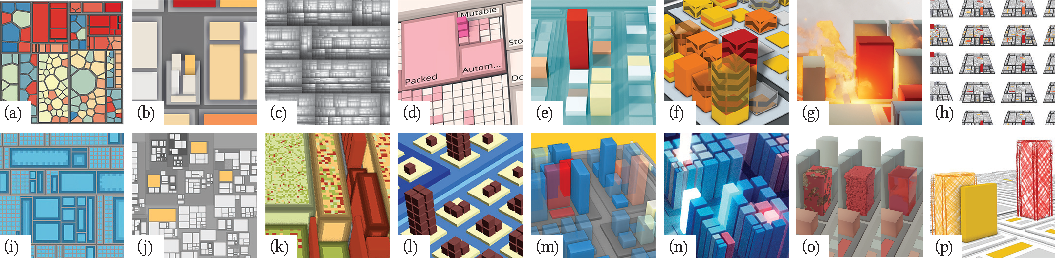
\includegraphics[width=\textwidth]{figures/teaser}
  \caption{
	A compilation of advanced software maps:
	(a) mixed use of rectangular and Voronoi layout,
	(b) mixed projection to combine 2D and 2.5D depictions,
	(c) structure-enhancing cushion shading,
	(d) visual aggregation for a higher-level view on the data,
	(e) a reference surface for improved height comparison and visual filtering,
	(f) in-situ comparison for different points in time,
	(g) using the fire metaphor to augment interpretability,
	(h) small multiples to compare multiple points in time and map themes,
	(i) different contour types to convey information on aggregated data,
	(j) using growing and shrinking to derive subsequent layouts,
	(k) color weaving to encode variation in underlying data,
	(l) subdivision on leaf nodes,
	(m) transparency as visual variable,
	(n) highlighting of nodes using glow,
	(o) rustiness, shininess, and
	(p) sketchiness as visual variable.
  }
  \label{fig:teaser}
\end{teaserfigure}

\maketitle

\section{Introduction}
\label{VINCI:Sec:Introduction}
\begin{figure*}[t]
	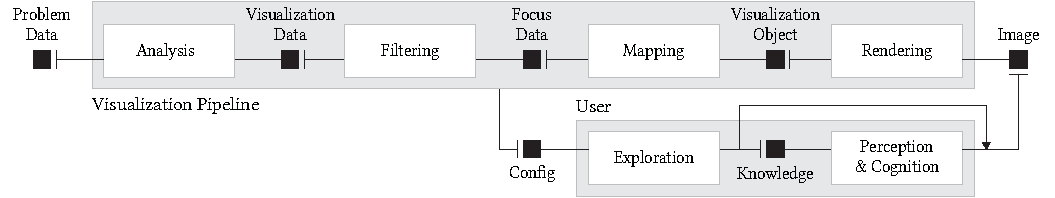
\includegraphics[width=\textwidth]{figures/vis-process-7}
	\caption{Model of the visualization process~\cite{wijk2005-visualization} consisting of a visualization pipeline~\cite{santos2004-gaining} and a feedback loop for knowledge gathering and interactive user control. 
		This model is applicable to visual software analytics using software maps.}
	\label{fig:visualization-process}
\end{figure*}
\par
Treemaps are an established information visualization technique that implements the information seeking mantra~\cite{shneiderman1996-eyes} and is used in different domains~\cite{shneiderman2009-treemaps}.
They allow for a depiction of non-spatial, multivariate data and provide the convenience and expressiveness of thematic maps, \ie given a spatialization strategy (layouting), they support a combination of two or more visual variables for information display, such as color, size, or texture~\cite{carpendale2003-considering}.
The 2D depiction is often extended into the third dimension, resulting in so-called 2.5D treemaps, allowing for additional information display~\cite{turo1992-improve}.
2D~and~2.5D treemaps alike can support visual analytics to \enquote{foster the constructive evaluation, correction and rapid improvement of our processes and models and -- ultimately -- the improvement of our knowledge and our decisions}~\cite{keim2008-visual}.
\par
In the domain of software analytics, treemaps are used to depict software system data and software engineering data~\cite{wettel2007-comprehension,bohnet2011-codemonitoring}, resulting in so-called \emph{software maps}.
Software maps provide a unique and general-purpose interactive user interface and information display for software analytics tools.
Typically, a catalogue of \emph{software map themes} compiles commonly used attribute selections related to specific tasks in software analytics.
A software map theme, hereinafter referred to as \emph{map theme}, defines a selection of software information dimensions that are mapped onto visual variables of a software map.
It portrays selected aspects of the software information gathered and analyzed by software analytics processes.
A map theme presents, in a sense, topic-specific software map templates that support different stakeholders in software engineering in data-driven decision making as well as in finding actionable insights.
\par
To advance towards the goals of visual software analytics, \ie \enquote{(1) derive insight from massive, dynamic, ambiguous, and often conflicting data, (2) detect the expected and discover the unexpected, (3) provide timely, defensible, and understandable assessments, [and] (4) communicate assessment effectively for action}~\cite{keim2008-visual}, we derive the following challenges for software maps:
\begin{itemize}
	\item What are best practices and variations of software maps?
	\item How does the type of data impact its visualization?
	\item Can techniques be used individually or in combination?
	\item In what ways can data be depicted beyond the basic use of the visual variables position, area, height, and color?
\end{itemize}
\par
To provide a basis for answering these questions, we discuss advanced visual metaphors and techniques for software maps by exploring the visualization pipeline of software maps.
A superimposed visualization process integrates a visualization pipeline into a feedback loop with interactive user control of the various stages~\cite{wijk2005-visualization}.
Such a visualization pipeline is basically a sequence of three to four data processing stages with named inputs and outputs that conceptualize the transformation process of data into images.
This visualization process is well understood and there are only a few variations of models of visualization pipelines:
Using a data state reference model, the stages can be referred to as transformations, namely, (1) data transformation, (2) visualization transformation, and (3) view or visual mapping transformation~\cite{chi1998-operator,card1999-readings,chi2000-taxonomy}.
An extensive overview of specific transformations suitable for visualization purposes was recently provided by Liu~\etal~\cite{liu2017-advances}.
A similar naming scheme uses (1) data enrichment/enhancement, (2) visualization mapping, and (3) rendering to describe the same process~\cite{haber1990-visualization}.
This scheme was later refined to (1) data analysis, (2) filtering, (3) mapping, and (4) rendering~\cite{santos2004-gaining}.
For our purposes, we use the latter model and refer to the first two stages as \emph{preprocessing and filtering}.
\emph{Preprocessing and filtering} covers, among others, analytics, selection, enrichment, transformation, and resampling of raw data.
\emph{Mapping} maps abstract data to visual representations.
\emph{Rendering} creates a visual representation using image synthesis~(\cf~\autoref{fig:visualization-process}).
\par
Based on this approach, we provide an overview of advanced visual metaphors that have already been or can be used in combination with software maps to approach the above-mentioned challenges~(\cf~\autoref{fig:teaser}).
For it, we briefly summarize and discuss each metaphor and technique within the context of a stage within the conceptual model of the visualization pipeline and describe common practices based on our experiences.
We discuss the extent to which each metaphor or technique can be used to communicate different types of data and, furthermore, identify feasible combinations of isolated techniques and possible interferences, spanning as well as extending a design space of software maps.

\section{Design Space of Software Maps} %
\label{VINCI:Sec:DesignSpace}
\par
In software cartography, the term software maps is not uniquely defined. 
Each variation (such as software cities~\cite{wettel2007-comprehension}, code cities~\cite{wettel2008-codecity}, cityscapes, or thematic software maps~\cite{kuhn2008-thematicmaps}) focuses on its specific intended use, \ie visualizing abundant software system and process data and, thereby, providing a communication artifact for software engineering.
\enquote{A single graphic can convey a great deal of information about various aspects of a complex software system, such as its structure, the degree of coupling and cohesion, growth patterns, defect rates, and so on}~\cite{kuhn2008-thematicmaps}.
In order to obtain a more precise, low-level definition of \emph{software maps}, we propose a definition that precisely denotes them as a subset of treemaps using existing systematization approaches.
\par
Schulz \etal~\cite{schulz2011-implicit} identified the following axes for the design space of implicit hierarchy visualizations: dimensionality (either 2D or 3D), node representation (graphics primitives), edge representation (inclusion, overlap, and adjacency), as well as hierarchical layout (subdivision and packing).
D{\"u}bel \etal~\cite{duebel2014-2d3drepresentation} further differentiate between reference space and attribute space for a more precise classification -- assuming the validity of their classification is not affected by the non-spatial nature of treemaps.
\par
Using these design spaces, the software map can be expressed as follows.
For the spatialization of nodes of a software map we prefer subdivision or packing within a 2D reference space ($\mathcal{R}^2$).
The representation of edges is assumed to be implicit by means of nesting/inclusion.
Adjacency in 2.5D maps can also be used, but we suggest considering its use carefully; eventually we use flat representations of inner nodes only for all map themes in order to allow for special representation of aggregates.
Techniques that are based on containment and overlap in 3D are only marginally useful for medium to large data sets due to added interaction complexity and hard-to-resolve occlusion.
Fortunately, this restriction does not exclude any of the commonly used treemap layouting algorithms based on rectangular or Voronoi shapes~\cite{hahn2017-hybrid}.
\par
For the representation of leaf nodes, 2D graphics primitives are common, \eg Voronoi shapes or rectangles ($\mathcal{A}^2$).
They further can be extruded, optionally tapered, and thereby exploiting the third spatial dimension ($\mathcal{A}^3$).
\enquote{Increasing the visual vocabulary can provide for richer information resolution}~\cite{turo1992-improve} and allows for additional information display.
For these so-called 2.5D software maps, we generally prefer graphical primitives of rectangular footprints over more complex ones (\cf~\autoref{fig:voronoi-25d}) -- depending on (1) the importance of stability for the respective map theme and (2) whether or not rendering of more complex geometry is justifiable in terms of visual complexity, implementation complexity, and performance.
Since the reference space is still in $\mathcal{R}^2$, we support the term 2.5D~\cite{turo1992-improve} to avoid confusion with actual 3D treemaps that utilize a 3D layouting for positioning graphical elements in a 3D reference space ($\mathcal{R}^3$).
\par
With the attribute and reference space constrained, the typical characteristics of $\mathcal{A}^2\otimes\mathcal{R}^2$ and $\mathcal{A}^3\otimes\mathcal{R}^2$ visualizations adhere to software maps.
Consequently, we define software maps as a subset of 2D and 2.5D treemaps with the purposeful depictions of abstract software-system data and software engineering data, as well as software development data (\cf~\autoref{fig:overlay}).
This has one outstanding benefit: their characteristics largely match those of ubiquitously available, interactive 2D and 2.5D (geo-spatial) maps.
With this definition of software maps, both visualization engineers and software engineers can rely on and build upon well-established (1) interaction metaphors, (2) provisioning strategies, and (3) visualization metaphors, thereby harnessing the habits and experiences of most users.

\subsection{Data Characteristics}

Traditionally, visualizations targeting software analytics are required to handle three major aspects of software system data: static, dynamic, and evolving aspects~\cite{diehl2007-software}.
We use a broader scope for software maps by including software development data as well, which basically includes all stakeholders of the software development process.
The data typically covers mined, preprocessed data gathered from various sources:
\begin{itemize}
	\item Software implementations: Typically modularized and in distributed tree-structured components and source code units. In addition to topology information, additional metrics and other \emph{key performance indicators} (KPIs) are measured and derived by applying static source code analysis to the programmed artifacts (\eg source code, scripts, documentation).
	\item Dynamics of software executions (\emph{traces}): \eg analysis of run-time execution in order to capture a software's behavior.	
	\item Software development processes and evolution: \eg analysis of the engineering work on the system done by software developers. This is usually available in revisioning systems and issue, bug and customer feedback tracking tools.
\end{itemize}
\par
Even if measured exactly, the data is (1) prone to uncertainty due to missing semantic normalization, (2) lacks standardized metrics and interpretations, (3) is highly language-specific and, thus, highly heterogeneous in large software systems.
Further, anonymization may be required, the measurement resolution is unnecessarily high, and finally, the data is massive for medium- to large-sized engineering processes (metrics per file and per commit, plus all changes \wrt various issue tracking systems and continuous integration systems).
All these characteristics should be considered when specifying map themes or developing visualization techniques for visual information display using software maps.
An overview of visualization techniques for static aspects and their evolution, including visualization techniques besides treemaps and software maps, is listed in a survey by Caserta and Zendra~\cite{caserta2011-staticaspects}.
\begin{figure}[t]
	\centering
	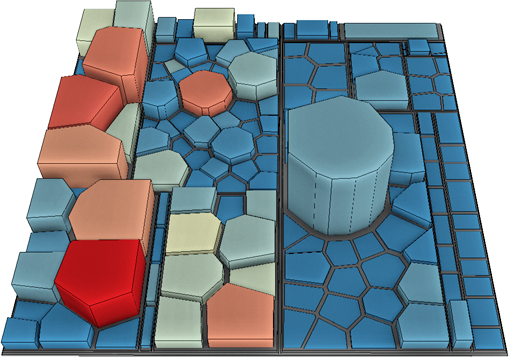
\includegraphics[width=1.0\linewidth]{figures/voronoi-25d}
	\caption{An example of a 2.5D software map with mixed use of rectangular and Voronoi treemap layouts.}
	\label{fig:voronoi-25d}
\end{figure}
\begin{figure}[t]
	\centering
	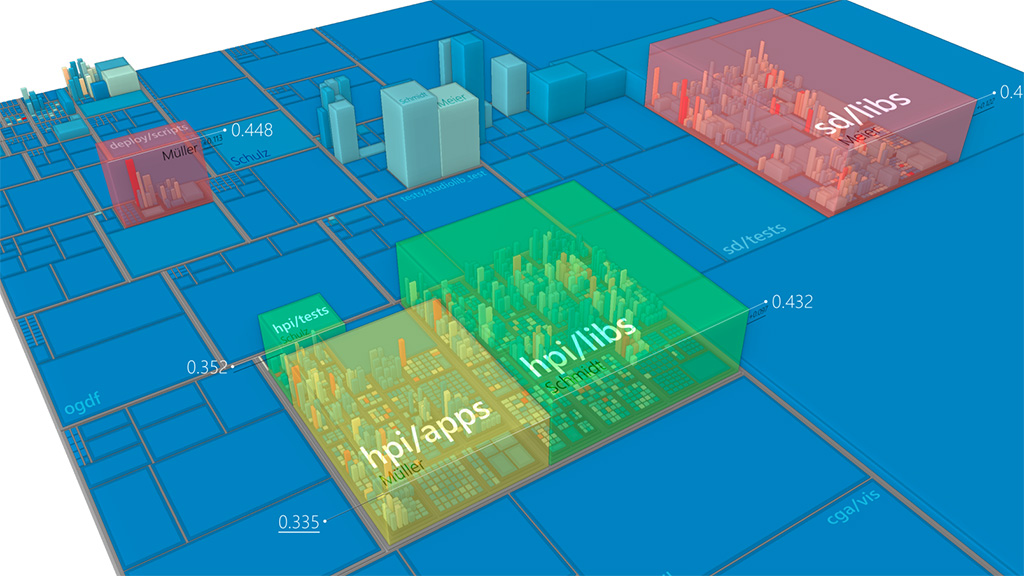
\includegraphics[width=1.0\linewidth]{figures/multi-semantic-treemap-cropped}
	\caption{An example of a semi-transparent information overlay to superimpose additional information.}
	\label{fig:overlay}
\end{figure}

\subsection{Preliminaries and Assumptions}
This paper does not provide a comprehensive set of common design guidelines for creating rectangular treemaps.
Guidelines concerned with perception~\cite{kong2010-guidelines} and use of color~\cite{schloss2018-colormap,xie2017-coloraesthetics,quinan2019-discretization} are outside the scope of this paper, since these are complex in themselves and still subject to active research.
The selection of presented visualization techniques focuses on visualization metaphors and techniques that cope with the data characteristics within the domain of software engineering, \ie volume and complexity of the data.
Thus, we selected visualization techniques that were used for software data and where an implementation can handle datasets up to hundreds of thousands of data items.
Contrarily, this paper does not cover city or city-like metaphors~\cite{knight1999-comprehension,balogh2015-codemetropolis} that map abstract data to features of virtual 3D city models such as building facades, car or pedestrian traffic, or street furniture.
Regarding frameworks and implementations of software maps, we refer to state-of-the-art approaches based on hardware acceleration and highly dynamic mappings~\cite{trapp2013-gputreemaps,scheibel2016-avcs}.
Similarly, the deployment and provisioning of data and visualization is highly contextual and application-specific~\cite{limberger2013-interactive,limberger2016-declarative3d}.
Fortunately, a simplifying view on the application scenarios allows deriving common characteristics and shared approaches for visualization~\cite{scheibel2019-hiviser}.

\section{Preprocessing and Filtering}
\label{VINCI:Sec:Preprocessing}
\par
During preprocessing and filtering, the incoming data -- also known as problem or task data -- is transformed and prepared for visualization.
This includes operations such as resampling, normalization, filtering of outliers, accumulating weighted leaf-node data to inner nodes, and more.
From a framework design perspective, we tend to leave any input data unmodified and let any transformation result in additional tree-structures and data views.
\paragraph{Attribute Resolution}
While creating software maps in practice, we encountered several challenges.
For example, the data is usually available in much higher resolution than required for visualization.
In those cases, we suggest reducing the data to a resolution that is reasonable for the map theme, \eg attributes mapped to area, color, or height do not require a \SI{32}{\bit} floating-point resolution.
Often, reducing the attribute resolution to a few bits can increase readability by means of discriminability and emphasize results of preceding data analysis.
This can also be supported from a perceptual point of view: height with perspective foreshortening is hardly comparable on a per-pixel basis and the exact size of a module within a treemap should be of subordinate relevance.
Thus, often a transformation to a categorical data type such as \emph{irrelevant, low, medium, and high} (for color, height, or change) or \emph{lower-outlier, below average, average, above average, and upper-outlier} (for area) seems to be comparably or even more effective.
\paragraph{Streaming and Level-of-Detail}
The major challenge, however, is that industry software projects tend to be massive (in terms of number of modules, code units, metrics, or activities).
This is often ignored or only marginally covered in research but has significant impact on visualization design.
Software maps might be streamed on demand (node by node, slice by slice, \etc).
Loading millions of attribute values for nodes that should not even be depicted (\eg as they are out of scope or of sub-pixel size) can decrease responsiveness and result in visual clutter or memory shortages.
It is beneficial to have a highly customizable, interactive level-of-detail~\cite{elmqvist2010-aggregation,limberger2017-aggregation} (filtering and rendering) that allows for dynamic detail (\cf~\autoref{fig:stepwiseaggregation}),~\eg detecting source code duplicates, generated code, automated activities, and filter irrelevant areas such as third party code.
Furthermore, the software map should always support the concept of mental maps, \ie the overall landscape/spatial layout should not change due to a dynamic level-of-detail.
A particular technique to combine aggregated and detailed views in combination with reduced occlusion is the \emph{lifted map}~\cite{chaudhuri2009-selfadaptive}.
\begin{figure}[tb]
	\centering
	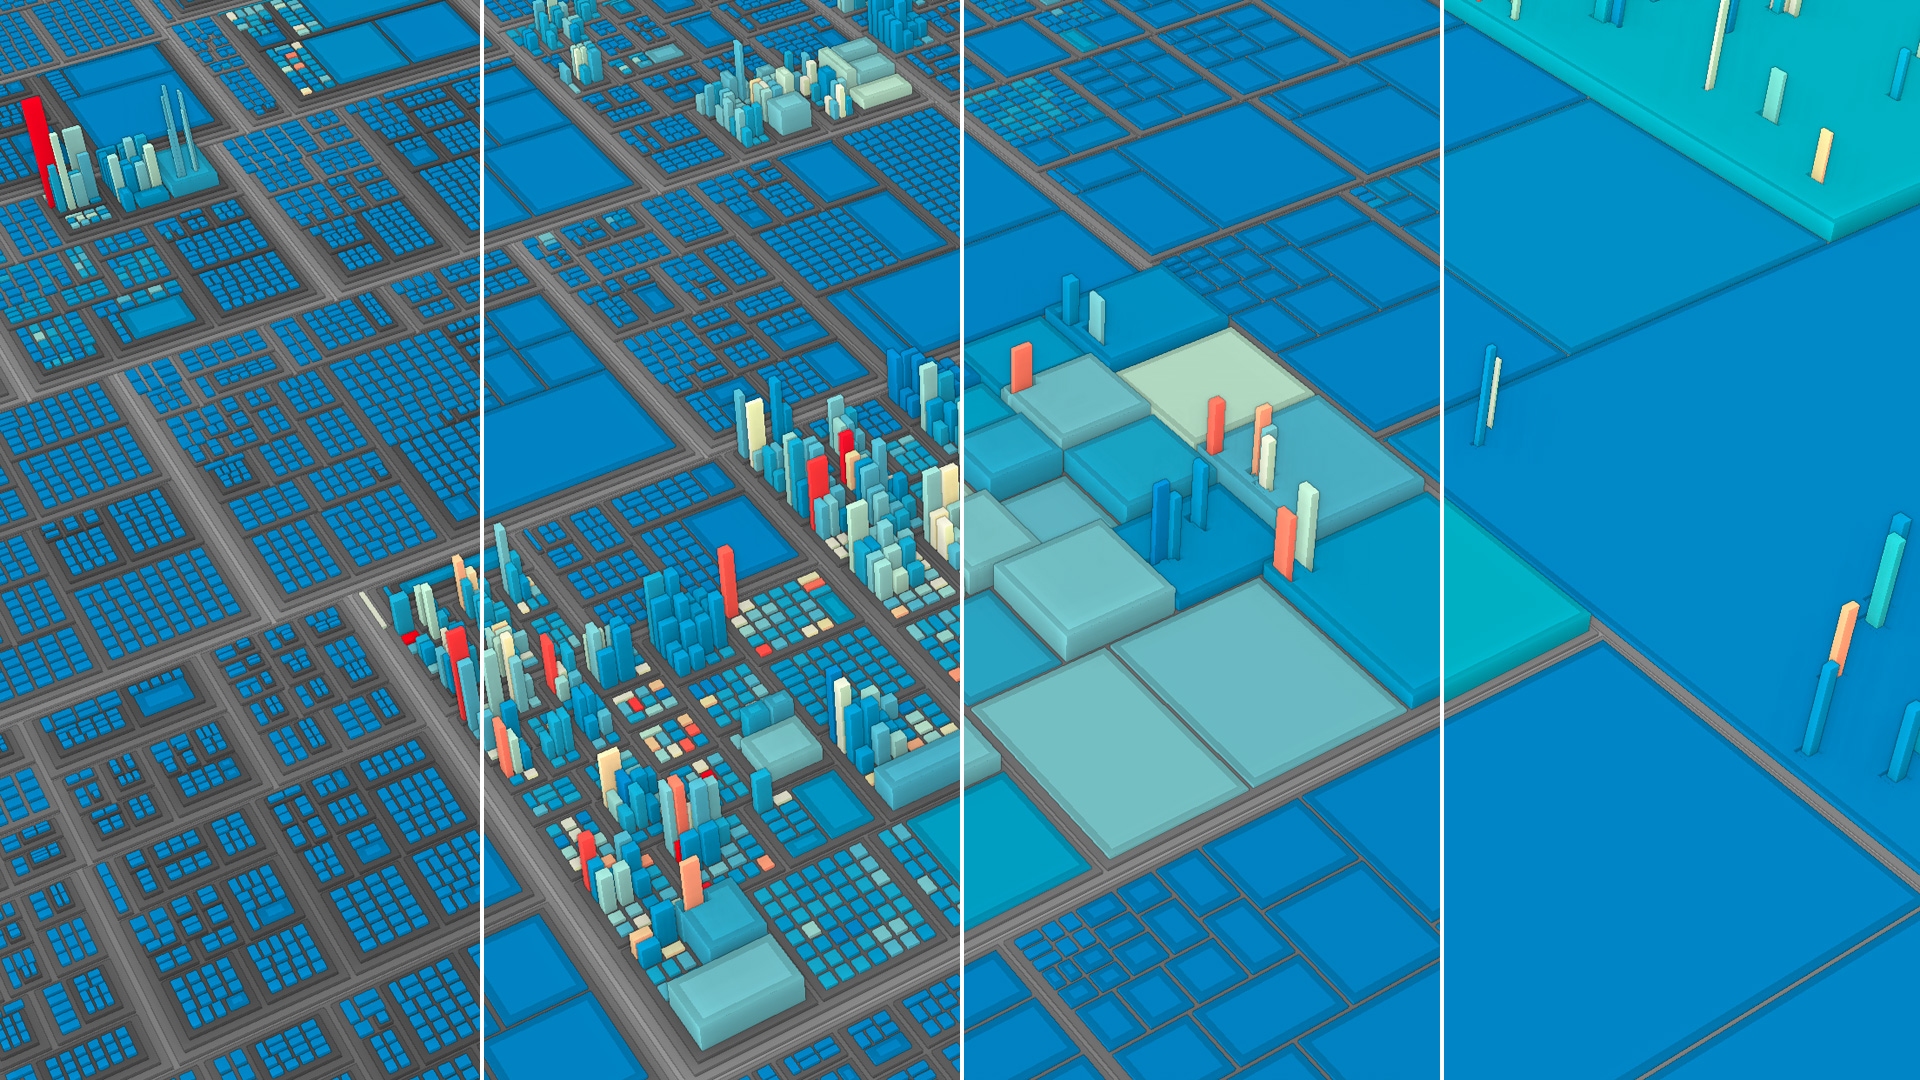
\includegraphics[width=1.0\linewidth]{figures/aggregation-w-outlier-stages}
	\caption{Stepwise generalization of a software map by use of aggregation, ranging from no aggregation (left) to strong aggregation (right).
		Outlier nodes -- also called landmarks -- are preserved~\cite{limberger2017-aggregation}.
	}
	\label{fig:stepwiseaggregation}
\end{figure}
\begin{figure*}[t]
	\centering
	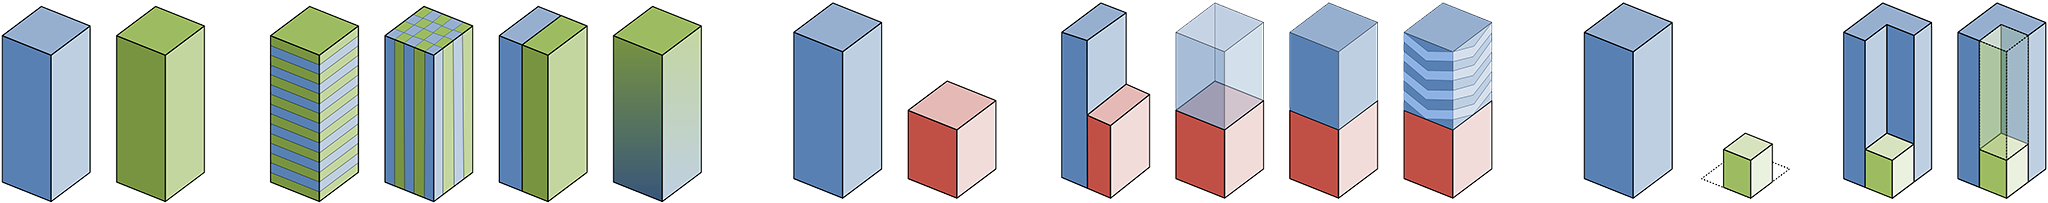
\includegraphics[width=\textwidth]{figures/in-situ-templates}
	\caption{A set of in-situ templates to depict changes in underlying data for up to three attributes using up to three visual variables~\cite{limberger2019-insitu}.
		Left group contains templates for color-only changes.
		Middle group contains templates for color and height changes.
		Right group presents templates for changes in all area, height, and color.
	}
	\label{fig:insitu}
\end{figure*}

\section{Mapping}
\label{VINCI:Sec:Mapping}
\par
The mapping stage transforms preprocessed and filtered data (\eg attribute values) into depictable and reversibly encoded graphical primitives and scenes.
This is a fundamental step for efficient encoding of input data and should address human capacities and abilities to decode a depiction~\cite{ware2012-information}.
There is not necessarily an explicit representation of the resulting visualization object in memory.
The result may only be volatile during visualization, especially from an implementation point-of-view: the distinction between mapping and rendering sustains more on a conceptual level~\cite{trapp2013-gputreemaps,scheibel2016-avcs}. 
\par
Software maps usually use inner nodes to depict applications, modules, or even source code units, \ie source code files~\cite{bohnet2011-codemonitoring}.
The leaf nodes each depict either modules, source code units, functions, events, developers, or activity (by means of commits).
The position of each node is computed by a layout technique specified by the map theme, and a metric is usually mapped to the size of the graphical primitive, \eg lines-of-code, file size, or size of domain logic.
\paragraph{Use of Height}
We utilize height of cuboids by means of an extrusion of the 2D shape~\cite{bladh2004-threedimensions,choi2011-stratatreemaps} as a secondary visual variable.
The idea is to provide the following order with declining importance for the task: (1) color, (2) height, (3) other visual variables.
For 2.5D software maps, pyramid-like shapes can be used to further encode an attribute or just reduce occlusion~\cite{turo1992-improve}.
When depicting evolving data with accustomed map themes, height seems to allow for an intuitive encoding of data changes by means of growing/increasing vs. shrinking/decreasing.
Height should not be used, however, to depict negative or diverging scales directly, as this would result in downwards facing cuboids.
Even though this was suggested several times, we prefer to refine the map theme to transform or map relevant value ranges of attributes to make a salient but expected use of visual variables (cuboids are high if data is of interest).
In contrast thereto, if a negative value range is relevant, it is mapped inversely to height. If positive values are relevant as well, the absolute value could be mapped to height and the sign to color, shape, or texture.
Finally, the orientation of the leaf node's geometry~\cite{langelier2005-qualityanalysis} and the type -- by means of poly cylinders~\cite{marcus2003-softvis} and three-dimensional glyphs~\cite{boccuzzo2007-cognitive} are further suitable as visual variables.
\paragraph{Evolutionary Data}
One of the biggest challenges for treemaps -- and thus, software maps -- is the handling of topology changes, \ie addition, move, and removal of nodes, in a predictable and comprehensible manner.
If the time range of interest is in the past, a multi-revision hierarchy can be computed~\cite{tu2007-changes}.
The quality of this hierarchy heavily depends on the computation's capabilities to track nodes over multiple revisions (renames, copies, clones, splits, moves, deletions, \etc).
If the software map is used to visualize ongoing processes and continuously evolving data, an initial layout can be incrementally evolved based on the topology changes, resulting in nodes growing, shrinking, appearing, and disappearing~\cite{scheibel2018-evocells}.
\paragraph{Juxtaposing and Complex Shapes}
For visual display of multiple states or sub-elements, data vases, stacked cuboids, or fragmenting can be used.
In remembrance of stacked bar charts, the extruded polytopes can be subdivided in height, allowing for depiction of subcategories and their share on the overall height~\cite{itoh2006-networkintrusion,giereth2008-patentportfolios}.
This process can further be utilized, \eg to encode evolution by means of \emph{evolution segments}~\cite{steinbruckner2013-evolution} and \emph{data vases}~\cite{thakur2009-datavases}.
Small multiples can be used for \enquote{the comparison of multiple software map themes and revisions simultaneously on a single screen}~\cite{scheibel2016-smallmultiples}.
We found this especially useful for generation of an overview on as well as exploration and identification of map theme variations.
\paragraph{Depicting Relations}
For an emphasis of the topology \wrt the nested structure of nodes, cushion shading~\cite{vanwijk1999-cushion}, variations of margins or padding, as well as extruded, stacked inner nodes~\cite{bladh2004-threedimensions} can be applied.
If additional relations of nodes in addition to their tree-structured topology are of interest (\eg functional dependencies or often-coinciding changes during the development process), edges or edge bundles can be superimposed on software maps~\cite{holten2006-edgebundles,steinbeck2019-evostreets}.
This approach, however, is visually constrained by the number of depicted relations and data set size.
Superimposing relations by means of edges or tubes on top of 2.5D treemaps introduces additional clutter, occlusion, and visual complexity that is not inherent to the treemap metaphor.

\section{Rendering}
\par
In this stage, the visualization object is transformed into images using (real-time) image synthesis. 
Although the mapping stage is usually aware of the available visual variables and metaphors, it usually  only provides appropriate attribute values, descriptions of graphic primitives, and additional data for rendering.
As a result of the rendering stage, the mapped attributes should be visually encoded in the resulting image by use of visual variables, some of which are mapped by means of geometry, \eg position or extent.
\paragraph{Depicting Change}
Many software map themes are designed to facilitate understanding of the evolution of the underlying data sets.
This eventually requires visual comparison of (1) multiple visual variables for (2) multiple points in time over (3) large time ranges.
Therefore, Tu and Shen~\cite{tu2007-changes} introduced contrast treemaps.
Their approach could be applied within visual software analytics by encoding two different states of the attribute mapped to area and color.
It was conceptually extended by in-situ templates~\cite{limberger2019-insitu}, which allow for visual encoding of former and latter states on a per-cuboid basis for rectangular software maps~(\cf~\autoref{fig:insitu}).
Specifically, basic and more complex templates were introduced in order to depict changes in more than one visual variable simultaneously, including area, color, and height.
Although not discussed in the paper, the templates allow for comparison of additional per-node visual variables as well.
The visual quality and expressiveness also depends on the available rendering techniques, \eg procedural texturing and transparency are accounted for by several templates.
\par
In practice, most of the comparison templates would result in a complex mapping and should be used for complex tasks or expert systems only.
For example, the depiction of area changes in combination with others is challenging to perceive.
However, they allow for a convenient encoding of changes in height that are usually mapped from secondary information such as number of authors, or size of domain logic.
Another use is to depict changes in color for primary information, \ie the most prominent indicator for the main purpose of the map theme, such as maintainability or faultiness of a software module.
\paragraph{Utilizing Textures}
Different texture patterns can be applied to encode categorical data~\cite{molli2001-multisynchronous}.
Exemplary attributes for texture pattern mapping are (the abstract) file type (\eg source code, documentation, deployment), associated teams, or budgets.
Alternatively, texture intensity was suggested as visual variable for scales with a natural zero~\cite{holten2005-realism}).
With most modern rendering engines supporting some form of physically based materials, textures can be used to enable visual variables based on their metalness or roughness (see natural metaphors).
In the past, we predominantly used procedural textures to depict quality measures (\eg degree of documentation, error-proneness), complexity measures (incoming or outgoing dependencies, mixed use of third-party dependencies), and development process indicators (\eg number of authors).
\paragraph{Utilizing Transparency}
Regarding geometric processing of inner nodes, there are approaches that extrude the layout as well, creating platforms~\cite{andrews1995-informationlandscapes} or pyramid frustums~\cite{andrews2002-informationpyramids}, placing child nodes \emph{on top} of the platforms.
Instead of stacking, there are approaches for nested depiction as well, \eg full spheres~\cite{balzer2004-softwarelandscapes} and hemispheres~\cite{balzer2004-largesoftware} in combination with transparency.
Other uses of transparency~\cite{luboschik2008-discovering} are (1) to reduce occlusion and (2) as a visual variable to encode different node states.
Transparency can further be used to depict removed or planned components, goals, irrelevant nodes as of the current map theme, or enhance the expressiveness and quality of (procedural) texturing.
However, the most relevant obstacle for using transparency is the complexity of its implementation: especially for web-based rendering clients, modern strategies such as order-independent transparency cannot easily be implemented due to limited graphics APIs and device capabilities.
One solution is to use stochastic dithering in a rendering framework based on multi-frame sampling~\cite{limberger2017-highqualityrendering}.
\begin{figure}[t]
	\centering
	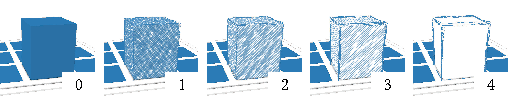
\includegraphics[width=\linewidth]{figures/2016-sketchy-stylization-order-pencil}
	\caption{A five-step scale to encode \enquote{uncertainty, imprecision or vagueness}~\cite{limberger2016-sketchy} using sketchiness as visual variable.
		The scale ranges from no uncertainty (left) to a high degree of uncertainty (right) with varying degrees of a sketch-rendering effect.
	}
	\label{fig:sketchiness}
\end{figure}
\paragraph{Depicting Uncertainty}
For the visual display of uncertainty, fuzzy drawing styles can be applied.
For example, node contour width as well as multiplexed frequency and amplitude could be parameterized~\cite{gortler2017-bubbletreemaps} and used to indicate vagueness.
Pencil-like outlines and hatching of surfaces can be combined into a single visual variable, \ie \emph{sketchiness} (\cf~\autoref{fig:sketchiness}).
Although technically an application of texture as a visual variable, mapping data to sketchiness is especially useful to encode \enquote{uncertainty, imprecision, or vagueness}~\cite{limberger2016-sketchy}.
Sketchiness is designed to encode varying degrees of uncertainty and, furthermore, can be used in addition to color.
For software maps, it can display measurement inaccuracies (incomplete or estimated data) or target data that is yet to be discussed or implemented (\ie targets for complexity, coverage, performance, or other quality measures).
\paragraph{Depicting Aggregates}
As previously discussed for the preprocessing and filtering stages, aggregation is an essential technique for software maps (\cf~\autoref{fig:aggregation}).
In the context of rendering, it is important to adhere to aggregation guidelines~\cite{elmqvist2010-aggregation}.
For example, the depiction should discern leaf nodes from aggregated ones.
In addition, small charts, diagrams, or glyphs encoding information of the underlying data can be expressed on top of or within aggregates~\cite{soares2018-adaptiveglyphs}.
Likewise, noise or color weaving~\cite{HaghShenas2006} as well as nesting-level contours (multiple contours that hint the depth of the aggregated sub-tree, \ie the number of an aggregate's subjacent hierarchy levels) can be used as well~\cite{limberger2017-aggregation}.
For software maps, the aggregation should summarize contextual data of low variation to provide orientation without distraction.
Aggregation can further extend user control and interaction, \eg by means of folding and unfolding, as well as for dynamically scaling the rendering load in order to comply with performance constraints.
\begin{figure}[t]
	\centering
	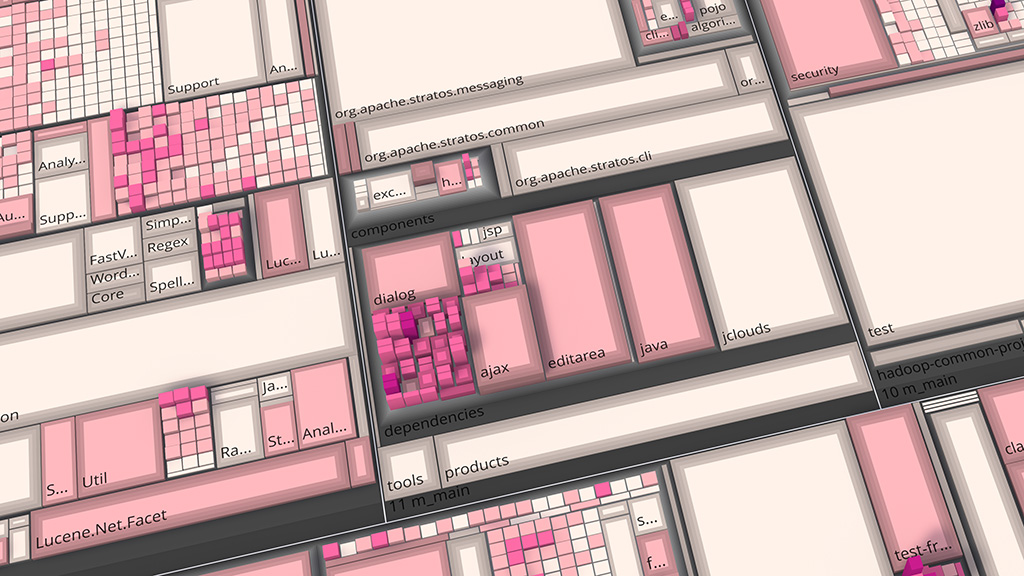
\includegraphics[width=1.0\linewidth]{figures/labeling}
	\caption{An example of software map aggregation and internal labeling~\cite{limberger2017-aggregation}.
		The resulting space from aggregating nodes is used to embed labels into the software map.
	}
	\label{fig:aggregation}
\end{figure}
\paragraph{Height-based Selection and Thresholding}
For 2.5D software maps, a reference surface -- a height reference -- can be used to \enquote{facilitate accurate identification of highest nodes as well as similar nodes~[\ldots]. It allows filtering and selection of nodes based on their height and depicts filtered and unselected notes in a clean way without introducing additional visual clutter.}~\cite{limberger2018-filtering}.
Depending on the capabilities of the renderer and the already occupied visual variables, one of various approaches for the visual display of the height reference can be applied, \eg intersection, stilts, explicit surface, closed surface, and implicit surface (\cf~\autoref{fig:referencesurfaces}).
Using user-controlled aggregation (by means of folding and unfolding) in combination with an interactive height-reference can provide a sufficient foundation for exploration-heavy tasks and map themes for single software maps and whole software map landscapes.
\paragraph{Using Natural Metaphors}
The use of natural metaphors is based on the idea that, \enquote{when faced with unfamiliar concepts, our cognitive system searches for the best mapping between the unknown concept and existing knowledge of other domains}~\cite{zhang2008-metaphors}.
To this end, natural metaphors, such as physically based materials (\eg rust, radiant emittance, roughness, and shininess; \cf~\autoref{fig:natural}) or weather phenomena (\eg rain, clouds, fire, dust, snow, \etc) were suggested to \enquote{emotionalize the visual communication by providing memorable visualizations}~\cite{wurfel2016-naturalphenomena}.
These metaphors can be used to depict change predictions or deviations from expected values on a secondary visual variable, while considering knowledge or best practices on preattentive processing of, \eg numerical information~\cite{few2004-tapping,hesse2017-preattentive}.
However, the use of weather phenomena requires sophisticated rendering techniques, renderers and an interactive context.
Further, their use might be inappropriate in certain professional contexts and even distracting for the map theme.
\begin{figure}[t]
	\centering
	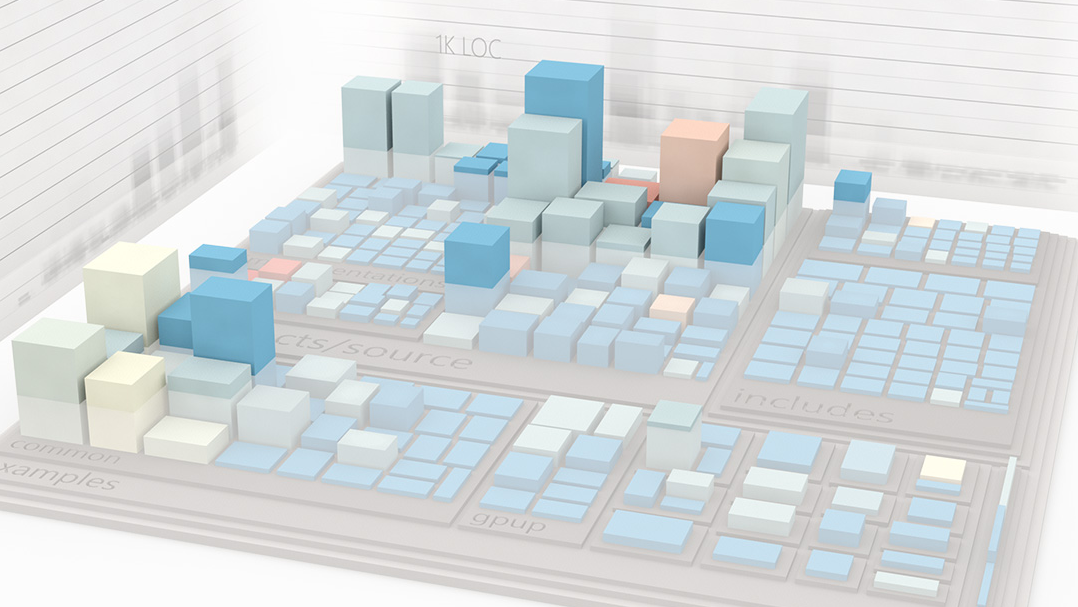
\includegraphics[width=1.0\linewidth]{figures/ref-surface-with-walls-cropped}
	\caption{An example combining visual filtering using a reference surface and adjacent charts that display per-axis projected height information~\cite{limberger2018-filtering}. The nodes that are below the reference surface are visually filtered by means of a semi-transparent surface metaphor.}
	\label{fig:referencesurfaces}
\end{figure}
\begin{figure}[t]
	\centering
	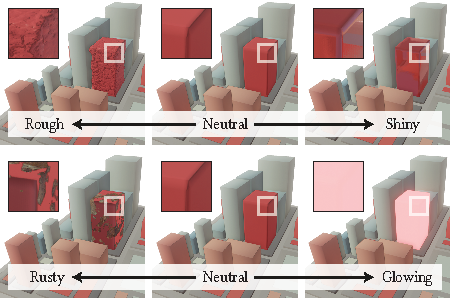
\includegraphics[width=1.0\linewidth]{figures/item-based-metaphors}
	\caption{An example of (top) rough-to-shiny and (bottom) rusty-to-glowing visualization metaphors to be used as visual variables.
		These metaphors are able to communicate deterioration or negative deviation (roughness, rust) and improvement or positive deviation (shine, glow) without need for further introduction of the mapping semantics~\cite{wurfel2016-naturalphenomena}.
	}
	\label{fig:natural}
\end{figure}
\paragraph{Mixed Projections}
Recently, an approach for focus-sensitive use of 2D and 2.5D treemaps was presented: 
\enquote{the technique operates by tilting the graphical elements representing inner nodes using affine transformations and animated state transitions}~\cite{limberger2017-mixed}.
This allows for on-demand separation of high-detail focus areas and context areas.
It further allows reducing occlusion issues -- which might occur for a certain data set or map theme -- and complexity of navigation (3D to 2D).
For software analytics, mixed projection can facilitate communication of the source code modules that are targeted for change in the current sprint.
In this example, the context is the other source code files present in the project.
Similarly, mixed projection can be of use if the height mapping is irrelevant for the context, but highly relevant for focus, \eg using the estimated time to invest for a source code module to be mapped to height.

\section{Conclusions and Future Work}
\par
This paper reviewed advanced visual metaphors and visualization techniques for software maps.
A brief discussion for each metaphor and technique is extended by common practices and own experiences of the authors.
Notably, the presented techniques are modular and can be used in combination in an on-demand manner without conflicting with other techniques.
This way, the software map can be used for a wide range of use cases.
Thereby, the approaches can visually scale from small to large and even massive data sets.
Summarizing, we argue that the software map is a highly versatile tool in visual software analytics.
\par
Future work will evaluate the applicability of the advanced metaphors and techniques to other 2D and 2.5D information visualization techniques.
In order to broadly provide the software map and its extensions, we plan to provide an open software ecosystem.

\begin{acks}
	This work was partially funded by the German Federal Ministry of Education and Research (BMBF) within the KMUi project \enquote{BIMAP} and the German Federal Ministry for Economic Affairs and Energy (BMWi) within the ZIM project \enquote{{Twin4Bim -- TASAM}}.
\end{acks}

\bibliographystyle{ACM-Reference-Format}
\balance
\bibliography{references}

\end{document}
\endinput
